\begin{document}


Two functions were created, both giving the temperature of a certain day. The difference is that one takes the date (month, day) as input and the other one takes the day number as input. To make it as simple as possible, the function that takes day number as input first coverts it into month and day, so that the functions after that is identical. 

The algorithm itself is straightforward. First, the dates in the data that matches the input date are found. Temperatures for every year is then stored in a vector, which is plotted in a histogram. A histogram for the 19$^{th}$ of July in Uppsala, for the years from 1722 to 2013, is shown in Fig. \ref{fig:tempOnDayNumber}.

\begin{figure}[h]
\begin{center}
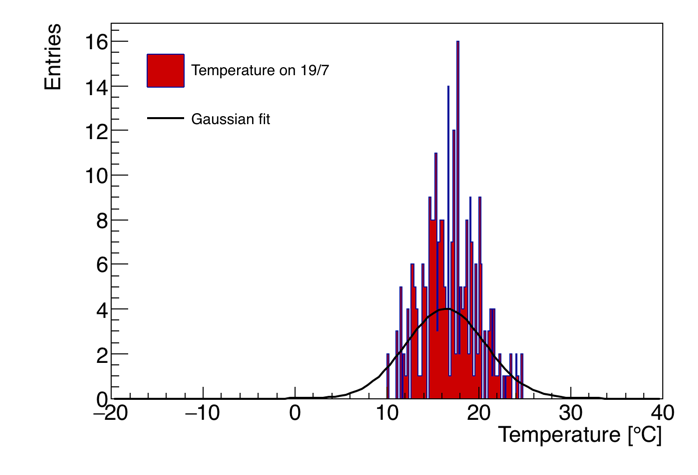
\includegraphics[scale=0.45]{tempOnDayNumber.png}
\caption{\label{fig:tempOnDayNumber} The temperatures on July 19$^{th}$ in Uppsala for the years between 1722 and 2013. The black line is a Gaussian fitted to the histogram.}
\end{center}
\end{figure}

From the histogram it is possible to get both the mean and the standard deviation. For Fig. \ref{fig:tempOnDayNumber}, the mean is 16.88 and the standard deviation is 2.96. If we want to know the probability for a certain temperature on the given day, we can use the mean and the standard deviation and assume a Gaussian distribution. The black line in Fig. \ref{fig:tempOnDayNumber} is a Gaussian fitted to the histogram, to see if it is a reasonable assumption. For Uppsala the data contains enough years to give 274 counts, so the Gaussian fit is sensible. Some of the other data sets would give a lot less data points, as in Fig. \ref{fig:tempOnDay}. The histogram contains only 35 entries for the 19$^{th}$ of July in Lund, and the Gaussian fit is not good. 

\begin{figure}[h]
\begin{center}
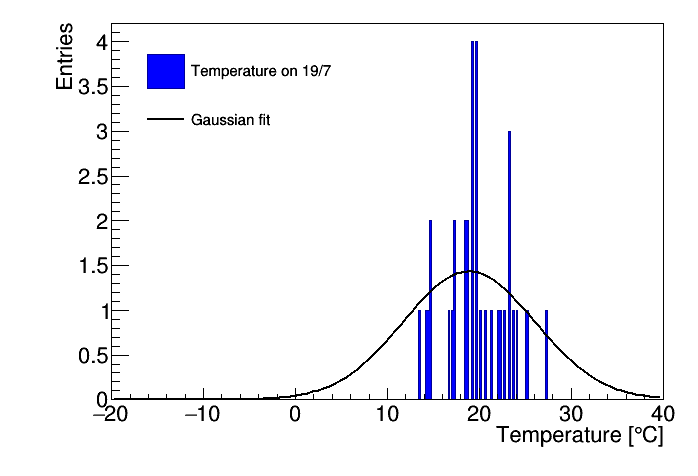
\includegraphics[scale=0.45]{tempOnDay.png}
\caption{\label{fig:tempOnDay} The temperatures on July 19$^{th}$ in Lund between 1961 and 2014. The black line is a Gaussian fitted to the data.}
\end{center}
\end{figure}

\begin{comment}
\begin{figure}[h]
\centering
\subfloat[Uppsala]{\label{fig:tempOnDayNumber2}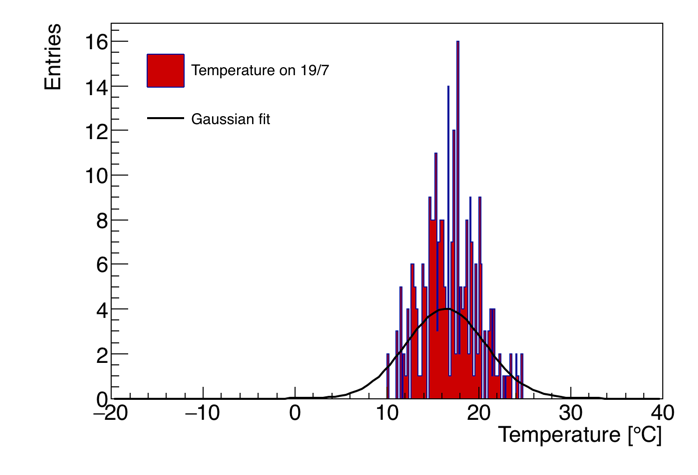
\includegraphics[width=0.5\textwidth]{tempOnDayNumber.png}} 
\subfloat[Lund]{\label{fig:tempOnDay2}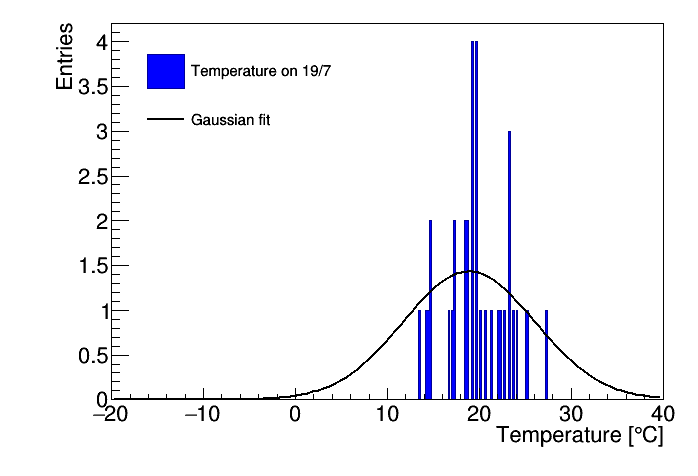
\includegraphics[width=0.5\textwidth]{tempOnDay.png}}\\
\caption{The temperatures on July 19$^{th}$ in Uppsala for the years between 1722 and 2013 in (a). The black line is a Gaussian fitted to the histogram.}
\label{fig:spring}
\end{figure}
\end{comment}


\end{document}